\documentclass[conference]{IEEEtran}
\usepackage{cite}
\usepackage{amsmath,amssymb,amsfonts}
\usepackage{algorithmic}
\usepackage{graphicx}
\usepackage{textcomp}
\usepackage{xcolor}
\usepackage{booktabs}
\usepackage{multirow}

\def\BibTeX{{\rm B\kern-.05em{\sc i\kern-.025em b}\kern-.08em
    T\kern-.1667em\lower.7ex\hbox{E}\kern-.125emX}}
\begin{document}

\title{Review Paper - An Image Is Worth 16X16 Words: Transformers for Image Recognition at Scale}

\author{\IEEEauthorblockN{Ashwin Chakravartula}
\IEEEauthorblockA{\textit{Institute for Data Science in Mechanical Engineering} \\
\textit{RWTH Aachen University}\\
Aachen, Germany \\
ashwin.chakravartula@rwth-aachen.de}
}

\maketitle

\begin{abstract}
While the Transformer architecture has become the de facto standard for natural language processing tasks, its applications to computer vision remain limited. The authors tried to show that the reliance on CNN s is not necessary and a pure transformer applied directly to sequences of image patches can perform very well on image classification tasks.
\end{abstract}

\begin{IEEEkeywords}
Vision Transformer, Inductive bias, CNNs
\end{IEEEkeywords}

\section{Introduction}
With this paper, the researchers are looking at different ways to perform general computer vision tasks, which do not necessarily involve the standard architecture. Vision-related tasks in computer vision help the machine to interpret and understand visual information. It consists of image classification, object detection, semantic segmentation \& Image generation and video understanding.

If we look into a typical CNN architecture, instead of specifically hand-designed feature detectors, the features are learned using deep neural networks and the features of input image are extracted in a hierarchical manner, and the output of this network is a classifier which gives us scores on what can the input image be best classified into.

CNNs have been state-of-the-art for quite some time, and especially with the skip-connections and residual networks, it has become easier to retain the high-resolution information, hence better classification. Some researchers have tried to combine CNN-like architectures with self-attention (Wang et al., Carion et al.) however theoretically efficient, have some scaling issues on modern hardware accelerators due to specialized attention patterns. The transformers use a self-attention mechanism, which has a computation that grows quadratically. While providing the input image directly to the self-attention block, in order to compute the attention scores, the mechanism needs to perform pixel-wise quadratic computation, which is not an efficient way of computing. Therefore, in large-scale image recognition, classic ResNet-like architectures are still state of the art (Mahajan et al., Xie et al., Kolesnikov et al.). The idea of using the self-attention mechanism in images was inspired by the success of using self-attention mechanism for NLP applications. The dominant approach is to pretrain the model with a large dataset of text and then fine-tune it on a smaller task-specific dataset. Because of transformers, its now feasible to train the model on huge datasets in a computationally efficient way, also proving that transformers are scalable. 
 

\section{Preliminaries}

\subsection{Transformer architecture}

The transformer architecture, initially proposed by Vasawani et al. for natural language processing (NLP) tasks, forms the basis of Vision Transformers. A transformer primarily consists of the following key components:
\begin{itemize}
\item Multi-head self-attention - For an input matrix \( X \in \mathbb{R}^{n \times d} \) (where \( n \) is the sequence length and \( d \) is the dimensionality of each token), self-attention is computed as:
\begin{equation}
\text{Attention}(Q, K, V) = \text{softmax}\left( \frac{QK^\top}{\sqrt{d}} \right)V    
\end{equation}
\item 
where \( Q, K, V \) are the query, key, and value matrices, obtained by linear transformations of \( X \).

\item Feedforward network - Each transformer block contains a position-wise feedforward network applied independently to each token: 
\begin{equation}
    \text{FFN}(x) = \text{ReLU}(x W_1 + b_1) W_2 + b_2
\end{equation}
\item Positional Encoding - Transformers do not have built-in notion of sequence order, therefore positional encodings are added to the input embeddings to inject information about token positions. In NLP, sinusoidal functions are often used, whereas Vision Transformers (ViTs) employ learnable position embeddings. 
\end{itemize}

\subsection{Inductive Bias}
\begin{itemize}
    \item Inductive bias is the model's built-in preference or assumptions that influence how it generalizes from it's training data to new unseen data.
    \item Since a model will always have limited training data, it uses inductive bias to fill in gaps by favoring certain kinds of patterns or relationships over others.
    \item So a model's inductive bias highly influences its generalization ability.
    \item Appropriate inductive bias helps the model in learning the true underlying structure of data.
    \item It also reduces overfitting as inductive bias acts as a form of regularization.
\end{itemize}


Since a model will always have limited training data, it uses inductive bias to fill in gaps by favoring certain kinds of patterns or relationships over others.


\begin{figure}[htbp]
\centerline{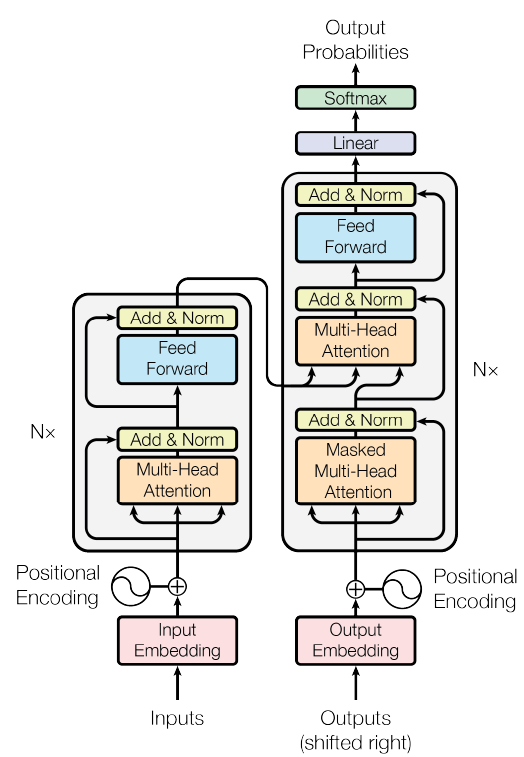
\includegraphics[width=0.5\linewidth]{transformer_architecture_MHSA.png}}
\caption{Transformer architecture showcasing multi-headed self-attention mechanism}

\end{figure}

\section{Problem Statement}
The implementation of self-attention mechanism in Computer Vision related tasks was only theoretically efficient, as it was found out that it was not scaled effectively on modern hardware accelerators due to the use of specialized attention patterns. The computational overhead of a vanilla transformer grows quadratically with respect to sequence length acting as a bottleneck for transformers to handle long sequences. This is because, each token in input sequence attends to every other token creating a dependency between all pairs. For a sequence of length N, there are N X N interactions to compute (N X N matrix of attention scores). This scaling makes computation and memory requirements increase rapidly as sequence length grows leading to high overload for longer inputs.

It means that the same model cannot be applied to the images where this computation would go pixel wise, hence the scalability issue. This was also one of the reasons why ResNets were still used as state-of-the-art methods to perform Computer vision tasks.

\section{Vision Transformer model}

\begin{figure}[htbp]
\centerline{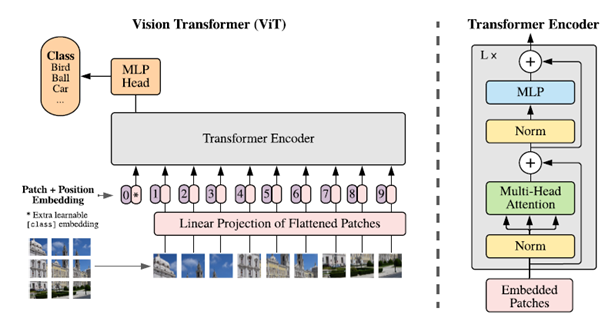
\includegraphics[width=0.75\linewidth]{vit_block.png}}
\caption{Vision Transformer architecture}

\end{figure}


\subsection{Model description}
ViT receives 2D image patches as an input instead of a standard 1D sequence of token embeddings. The patches are transformed into a lower dimensional numerical embedding using a Fully Connected Network (FCN), which acts as the input to the transformer encoder.

The transformer encoder consists of alternating layers of multiheaded self-attention and Multilayer Perceptrons (MLP) blocks in addition to it, each block consists of a LayerNorm and residual connections. [1]

There is also a classification token which is added to the sequence of embedded patches similar to bi-directional encoder representations from transformers. 

\begin{align}
z_0 &= [x_{\text{class}}; x_p^{1}E; x_p^{2}E; \ldots ; x_p^{N}E] + E_{\text{pos}}, \nonumber \\
& E \in \mathbb{R}^{(P^2 \cdot C) \times D}, \quad E_{\text{pos}} \in \mathbb{R}^{(N+1) \times D}
\end{align}

\begin{equation}
z_l^{'} = \text{MSA}(\text{LN}(z_{l-1})) + z_{l-1}, \quad l \in \{1, \ldots, L\}
\end{equation} 

\begin{equation}
z_l^{l} = \text{MLP}(\text{LN}(z_{l}^{'})) + z_{l}^{'}, \quad l \in \{1, \ldots, L\}
\end{equation}

\begin{equation}
y = \text{LN}(z_L^{0}) \quad l \in \{1, \ldots, L\}
\end{equation}



\subsection{Working principle of ViT}

The input 2D image is divided into smaller patches, such that each patch has a resolution of 16X16 pixels.
The vectors resolved from each of the patch images are converted into input embeddings once they pass through FCNs. These embeddings help projecting data into vector space.
Positional encodings are added to input embeddings before it gets processed by Transformer encoder.

\begin{figure}[htbp]
\centerline{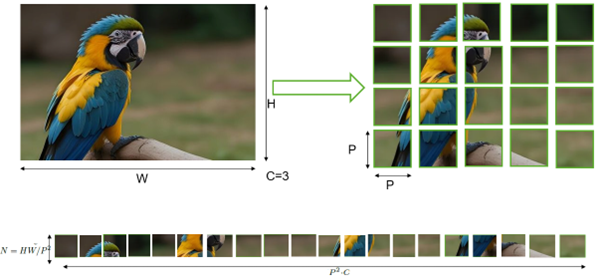
\includegraphics[width=1\linewidth]{vit_16_16_mechanism.png}}
\caption{ViT mechanism describing the patch creation from the input image}

\end{figure}

\subsection{CLS Token}
The reason why CLS tokens are used is to get a single global representation from the multiple embeddings at the input.
Out of all the vectors resolved from each of the patch images, there's one additional input which is the class token; it's a dummy input which is initially filled with random values but is a learnable vector which gets updated iteratively.



\subsection{Positional encoding}
Positional encodings are learnable vectors which are added to the patch embeddings to provide the model with information about the spatial layout of patches, since transformers lack inherent knowledge of sequence/ positions.
These position embeddings can be trained during model optimization, and each position gets its own embedding.

Position encoding can also be fixed, for example. such as sine and cosine functions of different frequencies can be used to generate these encodings.


\section{Experiment}

A comparison is made between different kinds of architectures (explain which ones)
In order to do this, representation learning capabilities of ResNet, Vision Transformer, and hybrid architectures are compared. It was observed that while considering the computational cost of pre-training the model, ViT performs very favorably, attaining state of the art on most recognition benchmarks at a lower pre-training cost.

\subsection{Setup}


Model's scalability is explored using different datasets with increasing amount of classes and images such as ILSVRC-2012 ImageNet dataset with 1k classes and 1.3M images, ImageNet-21k with 21k classes and 14M images (Deng et al. 2009), JFT (Sun et al. 2017) with 18k classes and 303M high-resolution images.

The models trained on these datasets are transferred to several benchmark tests such as CIFAR - 10/100, Oxford-IIIT Pets, Oxford Flowers-102, and VTAB Classificaion suite.


\begin{table}[htbp]
\centering
\caption{Details of Vision Transformer model variants.}
\label{tab:vit_model_variants}
\begin{tabular}{lccccc}
\toprule
\textbf{Model}     & \textbf{Layers} & \textbf{Hidden size $D$} & \textbf{MLP size} & \textbf{Heads} & \textbf{Params} \\ 
\midrule
ViT-Base           & 12              & 768                      & 3072              & 12             & 86M             \\ 
ViT-Large          & 24              & 1024                     & 4096              & 16             & 307M            \\ 
ViT-Huge           & 32              & 1280                     & 5120              & 16             & 632M            \\ 
\bottomrule
\end{tabular}
\end{table}


Three different model configurations of ViT were used which were directly adopted from BERT. The authors also added the "Huge" model and addition to the existing two models "Base" and "Large".
It was also observed that Transformer's sequence length is inversely proportional to the square of patch size, which means that models with smaller patch size are computationally more expensive.
The authors used ResNets for baseline CNNs (He et al. 2016), but replaced Batch normalization layers with Group normalization (Wu and He, 2018), and used standardized convolutions and named the above modified block as ResNet (BiT). 

For creating the hybrid architecture, the authors fed the intermediate feature maps of ResNets into ViT with patch size of one “pixel”. 



\subsection{Comparison of setup with state of the art}
The authors compared the largest models - ViT H/14 and ViT-L/16 to the state of the art CNNs from the literature. 
For creating the hybrid architecture, the authors fed the intermediate feature maps of ResNets into ViT with patch size of one “pixel”. The authors selected comparison points with one using supervised transfer learning with large ResNets (Big Transfer – Kolesnikov et al., 2020) and semi-supervised transfer learning using trained EfficientNet model ie. Noisy Student (Xie et al.,). 

\begin{table}[htbp]
\centering
\small
\caption{Comparison with state of the art on popular image classification benchmarks.}
\label{tab:vit_model_comparison}
\resizebox{\columnwidth}{!}{%
\begin{tabular}{lccccc} 
\toprule
& \textbf{Ours-JFT} & \textbf{Ours-JFT} & \textbf{Ours-121k} & \textbf{BiT-L} & \textbf{Noisy Student (EfficientNet-L2)} \\ 
\midrule
\textbf{ImageNet}            & 88.55 $\pm$ 0.04 & 87.76  $\pm$ 0.03 & 85.30 $\pm$ 0.02 & 87.54 $\pm$ 0.02 & 88.4/88.5 *  \\ 
\textbf{ImageNet ReaL}       & 90.72 $\pm$ 0.05 & 90.54  $\pm$ 0.03 & 88.62 $\pm$ 0.05 & 90.54          & 90.55        \\ 
\textbf{CIFAR-10}            & 99.50 $\pm$ 0.06 & 99.42  $\pm$ 0.03 & 99.15 $\pm$ 0.03 & 99.37 $\pm$ 0.06 & -            \\ 
\textbf{CIFAR-100}           & 94.55 $\pm$ 0.04 & 93.90  $\pm$ 0.05 & 93.25 $\pm$ 0.05 & 93.51 $\pm$ 0.08 & -            \\ 
\textbf{Oxford-IIIT Pets}    & 97.56 $\pm$ 0.03 & 97.32  $\pm$ 0.11 & 94.67 $\pm$ 0.15 & 96.62 $\pm$ 0.23 & -            \\ 
\textbf{Oxford Flowers-102}  & 99.68 $\pm$ 0.02 & 99.74  $\pm$ 0.00 & 99.61 $\pm$ 0.02 & 99.63 $\pm$ 0.03 & -            \\ 
\textbf{VTAB (19 tasks)}     & 77.63 $\pm$ 0.23 & 76.28  $\pm$ 0.46 & 72.72 $\pm$ 0.21 & 76.29 $\pm$ 1.70 & -            \\ 
\textbf{TPUv3-core-days}     & 2.5k             & 0.68k             & 0.23k            & 9.9k            & 12.3k        \\ 
\bottomrule
\end{tabular}
}
\end{table}


In the above table, the mean and standard deviation of the accuracies, averaged over three fine-tuning runs were reported. 


\subsection{About VTAB Classification Suite}

\begin{itemize}
    \item VTAB stands for Visual Task Adaptive Benchmark; Its a diverse and challenging suite of tasks designed to evaluate general visual representations.
    \item It can also be used to evaluate techniques other than representation learning, that improve performance across a variety of tasks such as architectures, pre-processing function or optimizers.
    \item VTAB contains 19 tasks which cover a broad range of domains and semantics which are grouped into 3 sets : Natural, Specialized and Structured
    \item The Natural group represents classical vision problems and contain natural images captures using standard cameras. The classes may represent generic, fine-grained or abstract objects.
    \item The specialized group also contains images of the world, but captured through specialist equipment. The images have different invariances to those in the NATURAL tasks.
    \item The structured group assesses comprehension of the structure of a scene, for example, object counting or 3D depth prediction. 
    \item The teasks are generated from simulated environments, whose structure is easy for a human to determine, but whose domain differs greatly to datasets like ImageNet.

\end{itemize}


\subsection{Scaling study and pre-training data requirements}

To understand the importance of the dataset sizes, the authors performed Linear few-shot accuracy evaluation on ImageNet with respect to the pre-training size. 
For that, the models were trained on random subsets of 9M, 30M and 90M as well as the full JFT-300M dataset. 
To assess the intrinsic model properties, the authors didn't perform additional regularization on the smaller subsets and use the same hyper-parameters for all settings.
Fine-tuning accuracies capture the performance of each model after fine-tuning it on the respective dataset. Few-shot accuracies are obtained by solving a regularized least-squares regression problem that maps the frozen representations of subset of training images to target vectors.

\begin{table}[htbp]
\centering
\small % Adjust font size to match previous tables
\caption{Hyperparameters for fine-tuning.}
\label{tab:hyperparameter_tuning}
\begin{tabular}{lcc} 
\toprule
\textbf{Dataset}            & \textbf{Steps}  & \textbf{Base LR}                           \\ 
\midrule
ImageNet                    & 20,000          & \{0.003, 0.01, 0.03, 0.06\}                \\ 
CIFAR-100                   & 10,000          & \{0.001, 0.003, 0.01, 0.03\}               \\ 
CIFAR-10                    & 10,000          & \{0.001, 0.003, 0.01, 0.03\}               \\ 
Oxford-IIIT Pets            & 500             & \{0.001, 0.003, 0.01, 0.03\}               \\ 
Oxford Flowers-102          & 500             & \{0.001, 0.003, 0.01, 0.03\}               \\ 
VTAB (19 tasks)             & 2,500           & 0.01                                       \\ 
\bottomrule
\end{tabular}
\end{table}

 All models are fine-tuned with a cosine learning rate decay, a batch size of 512, no weight decay, and gradient clipping at global norm 1. If not mentioned otherwise, fine-tuning resolution is 384.
The authors fine-tuned all ViT models using SGD with a momentum of 0.9.  For fine-tuning ResNets and hybrid models the authors used the same setup, with the only exception of ImageNet where the authors added another value of 0.06 to the learning rate sweep.

\begin{table}[htbp]
\centering
\small
\caption{Performance comparison of ViT model variants across various datasets and pretraining sources.}
\label{tab:vit_details}
\resizebox{\columnwidth}{!}{%
\begin{tabular}{llccccc}
\toprule
\textbf{Dataset} & \textbf{Metric} & \textbf{ViT-B/16} & \textbf{ViT-B/32} & \textbf{ViT-L/16} & \textbf{ViT-L/32} & \textbf{ViT-H/14} \\ 
\midrule
\multirow{6}{*}{\textbf{ImageNet}} 
& CIFAR-10            & 98.13 & 97.77 & 97.86 & 97.94 & -   \\ 
& CIFAR-100           & 87.13 & 86.31 & 86.35 & 87.07 & -   \\ 
& ImageNet            & 77.91 & 73.38 & 76.53 & 71.16 & -   \\ 
& ImageNet ReaL       & 83.57 & 79.56 & 82.19 & 77.83 & -   \\ 
& Oxford Flowers-102  & 89.49 & 85.43 & 89.66 & 86.36 & -   \\ 
& Oxford-IIIT-Pets    & 93.81 & 92.04 & 93.64 & 91.35 & -   \\ 
\midrule
\multirow{6}{*}{\textbf{ImageNet-21k}} 
& CIFAR-10            & 98.95 & 98.79 & 99.16 & 99.13 & 99.27 \\ 
& CIFAR-100           & 91.67 & 91.97 & 93.44 & 93.04 & 93.82 \\ 
& ImageNet            & 83.97 & 81.28 & 85.15 & 80.99 & 85.13 \\ 
& ImageNet ReaL       & 88.35 & 86.63 & 88.40 & 85.65 & 88.70 \\ 
& Oxford Flowers-102  & 99.38 & 99.11 & 99.61 & 99.11 & 99.51 \\ 
& Oxford-IIIT-Pets    & 94.43 & 93.02 & 94.73 & 93.09 & 94.82 \\ 
\midrule
\multirow{6}{*}{\textbf{JFT-300M}} 
& CIFAR-10            & 99.00 & 98.61 & 99.38 & 99.19 & 99.50 \\ 
& CIFAR-100           & 91.87 & 90.49 & 94.04 & 92.52 & 94.55 \\ 
& ImageNet            & 84.15 & 80.73 & 87.12 & 84.22 & 88.03 \\ 
& ImageNet ReaL       & 88.85 & 86.27 & 89.99 & 88.28 & 90.33 \\ 
& Oxford Flowers-102  & 99.56 & 99.27 & 99.56 & 99.45 & 99.68 \\ 
& Oxford-IIIT-Pets    & 95.80 & 93.40 & 97.11 & 95.83 & 97.56 \\ 
\bottomrule
\end{tabular}
}
\end{table}


\section{Discussion and summary}

\begin{figure}[htbp]
\centerline{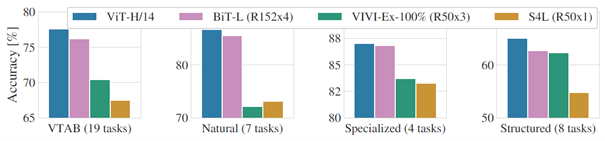
\includegraphics[width=1\linewidth]{vtab_performance_comparison.png}}
\caption{Breakdown of VTAB performance in Natural, Specialized and Structured task groups}

\end{figure}

It is observed that the Vision Transformer models pre-trained on the JFT-300M dataset outperform ResNet-based baselines on all datasets, while taking substantially less computational resources to pre-train.
ViT pre-trained on the smaller public ImageNet-21k also performed well.


\begin{figure}[htbp]
\centerline{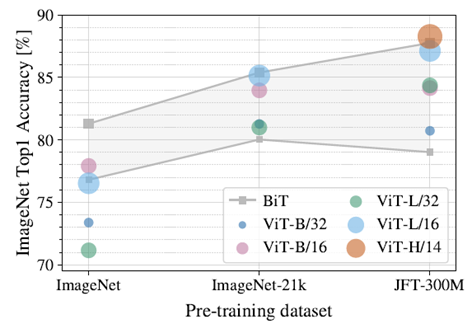
\includegraphics[width=1\linewidth]{imagenet_top_1_accuracy.png}}
\caption{Transfer to ImageNet. While large ViT models perform worse than BiT ResNets when pre-trained on small datasets, they show better performance when pre-trained on larger datasets. Similarly, larger ViT variants overtake smaller ones as the dataset grows.}

\end{figure}

\begin{figure}[htbp]
\centerline{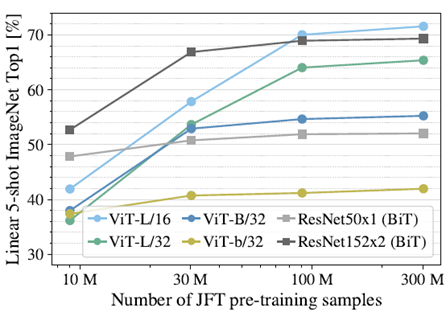
\includegraphics[width=1\linewidth]{linear_5_shot_accuracy.png}}
\caption{Linear few-shot evaluation on ImageNet versus pre-training size. ResNets perform better with smaller pre-training datasets but plateau sooner than ViT, which performs better with larger pre-training.}

\end{figure}

It is observed that Vision Transformers overfit more than ResNets with comparable computational cost on smaller datasets. For example, ViT-B/32 is slightly faster than ResNet50; it performs much worse on the 9M subset, but better on 90M+ subsets. The same is true for ResNet152X2 and ViT-L/16 which reinforces the intuition that the convolutional inductive bias is useful for smaller datasets.
However, it is also observed that for larger models, learning the relevant patterns directly from the data is sufficient, even beneficial.


\begin{figure}[htbp]
\centerline{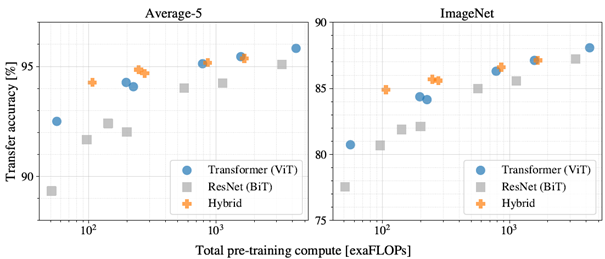
\includegraphics[width=1\linewidth]{transfer_accuracy_exaflops.png}}
\caption{Performance versus pre-training compute for different architectures: Vision Transformers, ResNets and hybrids.}

\end{figure}
As observed in Figure 7, Vision Transformers generally outperform ResNets with the same computational budget. Hybrids improve upon pure Transformers for smaller model sizes, but the gap vanishes for larger models.

ViT uses approximately 2 - 4x less compute to attain the same performance (average over 5 datasets). In addition to it, hybrid models slightly outperform ViT at small computational budgets, but the difference vanishes for larger models. This result is somewhat surprising, since one might expect convolutional local feature processing to assist ViT at any size.




Another interesting point of comparison to look into is the real-world speed of the architectures on the hardware, which is not always predicted well by theoretical FLOPs.
Figure 8 shows how many images can one core handle per second, across various input sizes. It is observed that the theorectical bi-quadratic scaling of ViT with image size only starts happening for the largest models at the largest resolutions. 

It is also observed from Figure 8 that large ViT models have a clear advantage in terms of memory-efficiency over ResNet models.

\begin{figure}[htbp]
\centerline{\includegraphics[width=1\linewidth]{wall_clock_timings_comparison.png}}
\caption{Left: Real wall-clock timings of various architectures across input sizes. Right: Largest per-core batch-size fitting on device with various architectures across input sizes.}

\end{figure}

Overall, the authors explored the direct application of Transformers for image recognition tasks. For bringing novelty, and to observe the pure data driven performance, image-specific inductive bias was not introduced to the architecture apart from the initial patch extraction step.

The image was interpreted as a sequences of patches and these patches were processed inside the Transformer encoder to get classification scores, similar to the ones used in NLP applications. It is concluded that this strategy works surprisingly well when coupled with pre-training on large datasets, thus it could be said that the Vision Transformers matches or even exceeds the state of the art on many image classification datasets, whilst being relatively cheap to pre-train.

\begin{thebibliography}{00}
\bibitem{b1} A. Dosovitskiy, L. Beyer, A. Kolesnikov, D. Weissenborn, X. Zhai, T. Unterthiner, M. Dehghani, M. Minderer, G. Heigold, S. Gelly, J. Uszkoreit, and N. Houlsby, "An Image is Worth 16x16 Words: Transformers for Image Recognition at Scale," arXiv preprint, arXiv:2010.11929, 2021. [Online]. Available: [https://arxiv.org/abs/2010.11929]
\bibitem{b2} Bello, B.Zoph, Q.Le, A. Vaswani, and J. Shlens. Attention augmented convolutional networks. In ICCV, 2019.
\bibitem{b3} Nicolas Carion, Francisco Massa, Gabriel Synnaeve, Nicolas Usunier, Alexander Kirillow, and Sergey Zagoruyko. End-to-end object detection with transformers. In ECCV, 2020.
\bibitem{b4} Mark Chen, Alec Radford, Rewon Child, Jeff Wu, and Heewoo Jun. Generative pretraining from pixels. In ICML, 2020a.
\bibitem{b5} Jean-Baptise Codonnier, Andreas Loukas, and Martin Jaggi. On the relationship between self-attention and convolutional layers. In ICLR, 2020.
\bibitem{b6} Alex Krizhevsky, Ilya Sutskever, and Geoffrey E. Hinton. Imagenet classification with deep convolutional neural networks. In NIPS, 2012.
\bibitem{b7} Prajit Ramachandran, Niki Parmar, Ashish Vaswani, Irwan Bello, Anselm Levskaya, and Jon Shlens. Stand-alone self-attention in vision models. In NeurIPS, 2019.
\bibitem{b8} Sergey Ioffe and Christian Szegedy. Batch normalization: Accelerating deep network training by reducing internal covariate shift. 2015.
\bibitem{b9} Niki Parmar, Ashish Vaswani, Jakob Uszkoreit, Lukasz Kaiser, Noam Shazeer, Alexander Ku, and Dustin Tran. Image Transformer. In ICML, 2018.
\bibitem{b10} Rewon Child, Scott Gray, Alec Radford, and Ilya Sutskever. Generating long sequences with sparse transformers. arXiv, 2019.
\end{thebibliography}
\vspace{12pt}

\section{Appendix}
\subsection{Information about Linear few-shot evaluation}
Linear few-shot accuracy evaluation is an approach used in tasks involving self-supervised learning, representation learning, or transfer learning to test the quality of learned representations by training a simple linear classifier on a small, labeled dataset while keeping the rest of the model frozen. \\
Few shot learning setup – in this case, only a limited number of labeled examples such as , few samples per class are provided for training the linear classifier. Some common few-shot scenarios involve 1-shot, 5-shot or 10-shot learning, where 1, 5 or 10 are the samples per class that are available. \\
For the evaluation of few-shot learning, the accuracy is measured on a separate test set to assess how well the linear classifier performs. High accuracy in few-shot indicates that the pretrained model has learned meaningful and generalizable features.

\begin{figure}[htbp]
\centerline{\includegraphics[width=1\linewidth]{5_shot_axial_attention_models.png}}
\caption{Performance of Axial-Attention based models, in terms of top-1 accuracy on ImageNet 5-shot linear, versus their speed in terms of number of FLOPs and inference time.}

\end{figure}


\subsection{Inspecting Vision Transformer}

Self attention mechanism in ViTs enable to integrate information across the entire image even in the lowest layers. For that, the point of interest is the computation of average distance in image space across which information is integrated, based on the attention weights. The attention distance is analogous to receptive field size in CNNs. This highly localized attention model is may serve a similar function as early convolutional layers in CNNs. Hence, it was also observed that the model attends to image regions that are semantically relevant for classification.


\begin{figure}[htbp]
\centerline{\includegraphics[width=1\linewidth]{attention_image_segmentation.png}}
\caption{Representative examples of attention from the output token to the input space.}

\end{figure}


\end{document}
